\chapter{Nombres entiers, \\ multiples, diviseurs}\label{ChNbEntiersMultDiv}
\begin{acquis} % enlever peut-être le lien internet
\begin{itemize}
\item trouver des diviseurs d'un nombre (et tous les diviseurs si ce nombre n'est pas trop grand);
\item trouver des multiples d'un nombre; 
\item décomposer un nombre en produits de facteurs premiers;
\item calculer avec des puissances;
\item calculer le PGCD de deux nombres entiers;
\item résoudre des problèmes nécessitant l'utilisation du PGCD;
\item calculer le PPMC de deux nombres entiers.
\end{itemize}
\end{acquis}

\activites



\begin{activite}[Diviseurs communs, PGDC]

\begin{partie}
 \begin{minipage}[c]{0.5\textwidth}
On veut paver une surface rectangulaire avec des carrés identiques et sans coupe. La longueur du côté des carrés est un nombre entier de centimètres.
 \end{minipage} \hfill%
 \begin{minipage}[c]{0.4\textwidth}
  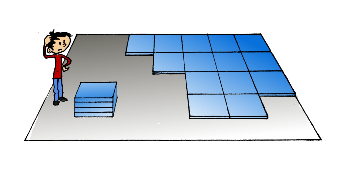
\includegraphics[width=4.8cm]{carrelage}
  \end{minipage} \\
 \begin{enumerate}
  \item La surface rectangulaire mesure 12 cm par 18 cm. Quelle peut être la longueur du côté des carrés ? Y a-t-il plusieurs possibilités ? Que représente(nt) ce(s) nombre(s) pour 12 et 18 ? Mêmes questions lorsque la surface rectangulaire mesure 49 cm par 63 cm, puis 27 cm par 32 cm et enfin 21 cm par 84 cm.
  \item Cherche les dimensions maximales d'un carré pouvant paver une surface rectangulaire de 108 cm par 196 cm.
  \end{enumerate}
\end{partie}

\begin{partie}
Un challenge sportif regroupe 30 filles et 75 garçons. Les organisateurs souhaitent composer des équipes comportant toutes le même nombre de filles et le même nombre de garçons. Comment peux-tu les aider pour qu'ils puissent constituer un nombre maximal d'équipes ? Donne ensuite le nombre de filles et de garçons dans chaque équipe. Explique ta démarche.
\end{partie}

\begin{partie}[PGDC]
\begin{enumerate}
 \item Dresse la liste des diviseurs de 30 et celle des diviseurs de 50. Quel est le plus grand diviseur commun à ces deux nombres ? On appelle ce nombre le \textbf{PGDC} de 30 et 50 et on le note : PGDC $(30 ; 50)$ ou PGDC $(50 ; 30)$.
 \item Quel est le PGDC de 8 et 24 ? Que remarques-tu ? Essaie de formuler une règle à partir de ce que tu as observé.
 \end{enumerate}
\end{partie}

\end{activite}

%%%%%%%%%%%%%%%%%%%%%%%%%%%%%%%%%%%%%%%%%%%%%%%%%%%%%%%%%%%%%%%%%%

\begin{activite}[Multiples communs, PPMC]

\begin{partie}
 \begin{minipage}[c]{0.6\textwidth}
Un engrenage est formé de 2 roues dentées $(A et B)$ qui ont respectivement 8 et 6 dents. Un point $R$ marqué sur une dent de la roue $B$ fait face à un point $S$ marqué entre deux dents consécutives de la roue $A$. On met l'engrenage en mouvement. Après combien de tours de la roue $A$ les points $R$ et $S$ seront-ils pour la première fois à nouveau dans la même position ? Même question lorsque la roue $A$ possède 9 dents et la $B$ 12 dents.
 \end{minipage} \hfill%
 \begin{minipage}[c]{0.2\textwidth}
  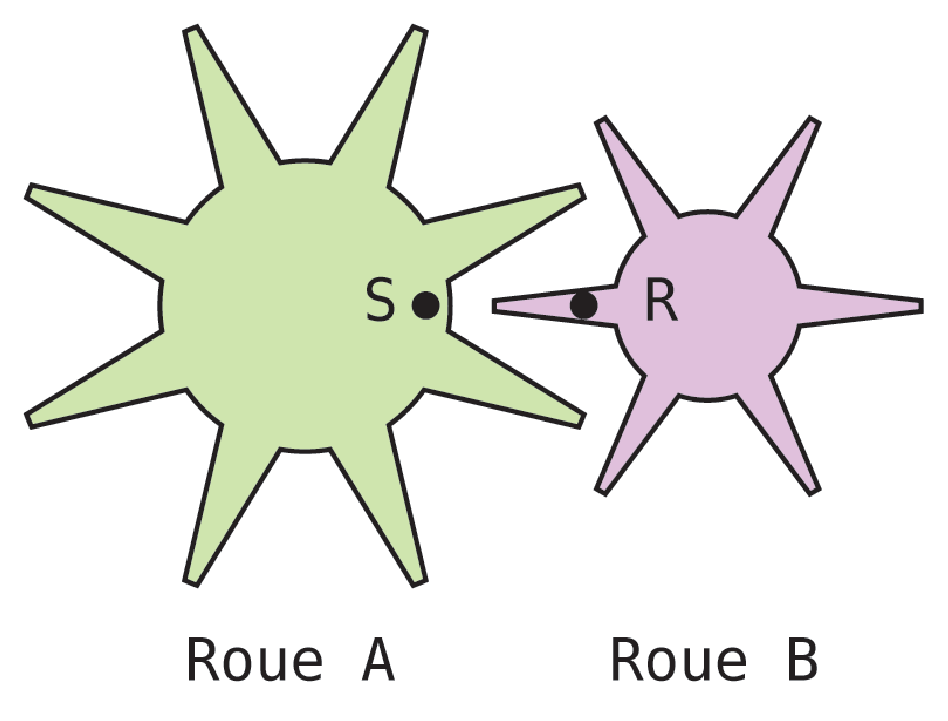
\includegraphics[width=3.8cm]{rouesAB}
  \end{minipage} \\
\end{partie}

\begin{partie}
Pendant l'été, un vendeur de glace ambulant visite le quartier de Jeannette tous les 7 jours et un autre vendeur de glace visite le même quartier tous les 5 jours. Quand les deux vendeurs sont présents le prix des glaces est diminué. Si les deux vendeurs de glaces ont visité le quartier aujourd'hui, quand sera la prochaine fois où le prix des glaces sera diminué ?
\end{partie}

\begin{partie}[PPMC]
\begin{enumerate}
 \item Dresse la liste des multiples de 9 et celle des multiples de 6. Quel est le plus petit multiple commun à ces deux nombres ? On appelle ce nombre le \textbf{PPMC} de 9 et 6 et on le note : PPMC $(9 ; 6)$ ou PPMC $(6 ; 9)$.
 \item Quel est le PPMC de 7 et 21 ? Que remarques-tu ? Essaie de formuler une règle à partir de ce que tu as observé.
 \end{enumerate}
\end{partie}

\end{activite}

%%%%%%%%%%%%%%%%%%%%%%%%%%%%%%%%%%%%%%%%%%%%%%%%%%%%%%%%%%%%%%%%%%

\newpage

\begin{activite}[Crible d'Eratostène]

 \begin{minipage}[c]{0.6\textwidth}
Ératosthène était un astronome, géographe, philosophe et mathématicien grec (276 – 194 av. J.-C.).
 \end{minipage} \hfill%
 \begin{minipage}[c]{0.2\textwidth}
  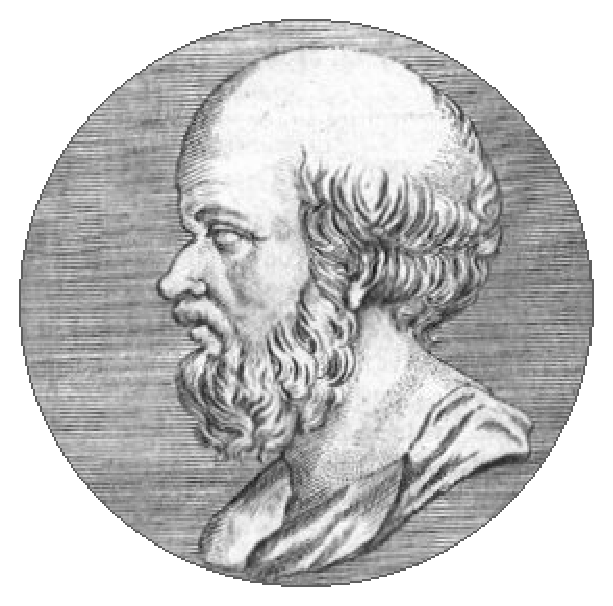
\includegraphics[width=3cm]{monnaie}
  \end{minipage} \\[1em]
  
\begin{tabularx}{1.01\linewidth}{|X|X|X|X|X|X|X|X|X|X|X|X|X|X|X|X|X|X|X|X|}
     \hline
     1 & 2 & 3 & 4 & 5 & 6 & 7 & 8 & 9 & 10 & 11 & 12 & 13 & 14 & 15 & 16 & 17 & 18 & 19 & 20 \\ \hline
     21 & 22 & 23 & 24 & 25 & 26 & 27 & 28 & 29 & 30 & 31 & 32 & 33 & 34 & 35 & 36 & 37 & 38 & 39 & 40 \\ \hline
     41 & 42 & 43 & 44 & 45 & 46 & 47 & 48 & 49 & 50 & 51 & 52 & 53 & 54 & 55 & 56 & 57 & 58 & 59 & 60 \\ \hline
     61 & 62 & 63 & 64 & 65 & 66 & 67 & 68 & 69 & 70 & 71 & 72 & 73 & 74 & 75 & 76 & 77 & 78 & 79 & 80 \\ \hline
     81 & 82 & 83 & 84 & 85 & 86 & 87 & 88 & 89 & 90 & 91 & 92 & 93 & 94 & 95 & 96 & 97 & 98 & 99 & \small{100} \\ \hline
  \end{tabularx} \\
  
\begin{enumerate}             
 \item Sur le tableau ci-dessus, entoure le chiffre 2 en rouge et raye tous les multiples de 2 autres que 2. Entoure le chiffre 3 en vert et raye tous les multiples de 3 autres que 3. Recommence avec le premier nombre non rayé et continue le processus jusqu'à ce que tous les nombres soient entourés ou rayés. Utilise des couleurs différentes pour chaque étape.
 \item Quelle est la particularité des nombres entourés ?
 \item Si on applique ce crible à tous les entiers naturels, 163 serait-il entouré ? Et 1\,678\,314 ?
 \item À l'aide du tableau, détermine les diviseurs de 24, 72, 17, 23 et 71.
 \end{enumerate}

\end{activite}

%%%%%%%%%%%%%%%%%%%%%%%%%%%%%%%%%%%%%%%%%%%%%%%%%%%%%%%%%%%%%%%%%%

\begin{activite}[Le triangle de Sierpinski]

\begin{partie}[Répondre avec des 3 et des $\times$ uniquement !]
\prof
{Dans la partie A, on se gardera d'utiliser la notation en puissances qui sera développée dans la partie B. Pour la question A2, on prendra soin d'écrire la multiplication du nombre 3, 7 fois puis 20 fois. Ainsi cela fera prendre conscience aux élèves comme s'est fastidieux et, de ce fait, l'intérêt de l'écriture en puissance.}
 \begin{minipage}[c]{0.5\linewidth}
La figure de départ est un triangle équilatéral rose. On construit à l'intérieur de celui-ci un triangle bleu obtenu en joignant les milieux des côtés du triangle de départ.
 \end{minipage} \hfill%
 \begin{minipage}[c]{0.4\linewidth}
 \begin{tikzpicture}	[scale=0.5]

%triangles de base
\filldraw [color=C3](0,0)--++(60:4)--++(-60:4)--cycle;
\filldraw [color=C3](5,0)--++(60:4)--++(-60:4)--cycle;

%triangles niveau 2
\fill [color=A2](7,0)--++(60:2)--++(180:2)--cycle;


\draw [->,>=stealth, very thick](3.5,2.5)--(5.5,2.5);
\node at(2,-0.5) {figure de départ};
\node at (7,-0.5) {figure 1};

\end{tikzpicture} 
  \end{minipage} \\[1.5em]
 
 \begin{minipage}[c]{0.2\linewidth}
 \begin{center} 
  \begin{tikzpicture}	[scale=0.5]

%triangle de base
\filldraw [color=C3](0,0)--++(60:4)--++(-60:4)--cycle;

%triangles niveau 2
\fill [color=A2](2,0)--++(60:2)--++(180:2)--cycle;

%triangles niveau 3
\fill [color=A2](1,0)--++(60:1)--++(180:1)--cycle;
\fill [color=A2](3,0)--++(60:1)--++(180:1)--cycle;
\fill [color=A2](2,1.74)--++(60:1)--++(180:1)--cycle;
   
\node at(2,-0.5) {figure 2};

\end{tikzpicture} 
 \end{center}
 \end{minipage} \hfill%
 \begin{minipage}[c]{0.74\linewidth}
  \begin{enumerate}
   \item De la même façon, on construit un petit triangle bleu dans chacun des triangles roses de la figure 1. Combien obtient-on de triangles roses dans la figure 2 ?
   \item Imaginons que l'on continue à construire des triangles bleus dans les triangles roses. Combien a-t-on de triangles roses dans la figure 4 ? Puis dans la figure 7 (en n'utilisant encore que des 3 et des signes $\cdot$ ) ? Et dans la figure 20 ?
   \end{enumerate}
  \end{minipage} \\[1em]
  
\end{partie}


\begin{partie}[Une nouvelle notation : la notation « puissance »]
La notation « puissance » est utilisée pour remplacer des produits comme dans les exemples suivants :
\begin{itemize}
 \item $9 = \stackrel{2 \text{ facteurs}}{\overbrace{3 \cdot 3}} = 3^2$ qui se lit « 3 au carré » ou « 3 puissance 2 » ou « 3 exposant 2 » ;
 \item $81 = \stackrel{4 \text{ facteurs}}{\overbrace{3 \cdot 3 \cdot 3 \cdot 3}} = 3^4$ qui se lit « 3 puissance 4 » ou « 3 exposant 4 ».
 \end{itemize}
\begin{enumerate}
 \item Écris, à l'aide de la notation « puissance », le nombre de triangles roses qu'il y a dans la figure 7 puis calcule ce nombre. Recommence pour la figure 20.
 \item À l'aide de ta calculatrice, indique combien il y a de triangles roses dans la figure 13, la figure 18, la figure 10 et enfin dans la figure 15. Existe-t-il un moyen d'effectuer ces calculs facilement avec ta calculatrice ?
 \end{enumerate}
\end{partie}

\end{activite}

%%%%%%%%%%%%%%%%%%%%%%%%%%%%%%%%%%%%%%%%%%%%%%%%%%%%%%%%%%%%%%%%%%

\begin{activite}[Des produits avec 2, 3 et 5]

Nous allons exprimer certains nombres sous la forme de produits. Dans cette activité, les seuls facteurs autorisés sont : 2 ; 3 et 5. Nous utiliserons la notation « puissance » dès que cela est possible.\\[0.25em]

 \begin{minipage}[t]{0.1\linewidth}
 \underline{Exemples} : 
  \end{minipage} \hfill%
 \begin{minipage}[t]{0.86\linewidth}
$25 = 5 \cdot 5$ peut s'écrire $25 = 5^2$ ;

$48 = 2 \cdot 2 \cdot 2 \cdot 2 \cdot 3$ peut s'écrire $48 = 2^4 \cdot 3$ ;

$90 = 2 \cdot 3 \cdot 3 \cdot 5$ peut s'écrire $90 = 2 \cdot 3^2 \cdot 5$.
 \end{minipage} \\

\begin{enumerate}
 \item Exprime de la même façon les nombres 4 ; 12 ; 27 ; 30 ; 45 et 108. Peut-on exprimer le nombre 26 de la même façon ? Justifie. \label{MbsEntMultDivis_acti1}
 \item Un élève a écrit l'égalité suivante : $54 = 2^1 \cdot 3^3$. En considérant que sa réponse est bonne, combien vaut $2^1$ ?
 \item Un élève a écrit l'égalité suivante : $50 = 2^1 \cdot 3^0 \cdot 5^2$. En considérant que sa réponse est bonne, combien vaut $3^0$ ?
 \item Réécris les trois exemples du départ puis les nombres de la question \ref{MbsEntMultDivis_acti1} sous la forme  $2^a \cdot 3^b \cdot 5^c$ (a, b et c sont des entiers naturels, éventuellement égaux à 0 ou 1).
 \item Trouve le plus possible de nombres inférieurs à 100 qui peuvent s'exprimer sous la forme d'un produit ne comportant que des 2, des 3 et des 5.
 \item Si maintenant les facteurs autorisés sont tous les nombres premiers. Exprime sous la forme d'un produit de facteurs premiers les nombres 42, 66, 198 et 990.
 \end{enumerate}
 
\end{activite}


\cours
\section{Multiples et diviseurs d'un nombre entier} 

% remarque : pour qu'un mot se retrouve dans le lexique : \MotDefinition{asymptote horizontale}{} 

\begin{aconnaitre}[Multiples et diviseurs]
\emph{12 $=$ 3 $\times$ 4}. On dit que :

\textcolor{C2}{\emph{12} est un multiple de \emph{3 (et de 4)}}

\textcolor{A1}{\emph{12} est divisible par \emph{3 (et par 4)}} ou \textcolor{J1}{\emph{3} est un diviseur de \emph{12}} ou \textcolor{H1}{\emph{3} divise \emph{12}}.
\end{aconnaitre}



%%%%%

\begin{methode*1}[Multiples, diviseurs]

\begin{exemple*1}
91 est-il un multiple de 7 ? 974 est-il divisible par 8 ? \\[1em]
\begin{minipage}[t]{0.46\linewidth}
$91 \div 7 = 13$ donc $91 = 7 \cdot 13$.

91 est donc un multiple de 7 (et de 13). On dit également que 91 est divisible par 7 (et par 13), que 7 est un diviseur de 91 (13 l'est aussi) ou que 7 divise 91 (13 divise aussi 91).
 \end{minipage} \hfill%
 \begin{minipage}[t]{0.46\linewidth}
 $974 : 8 = 121,75$.
 
121,75 n'est pas un entier, 974 n'est donc pas divisible par 8. On peut dire également que 8 n'est pas un diviseur de 974 et que 974 n'est pas un multiple de 8.
\end{minipage} \\

\end{exemple*1}

\exercice 
Établis la liste des diviseurs des entiers suivants : 60, 43 et 36.

\vspace{5em}


%\dotfill

%\dotfill

%\dotfill
%\correction

\exercice 
Détermine si 847 est un multiple de 7 :

%\dotfill

%\dotfill
%\correction

\end{methode*1}

%%%%%
  
\begin{aconnaitre}[Critères de divisibilité]
Un nombre entier est \textbf{\textcolor{A1}{divisible par 2}} si son chiffre des unités est pair (0, 2, 4, 6 ou 8) ;

Un nombre entier est \textbf{\textcolor{A1}{divisible par 3}} si la somme de ses chiffres est un multiple de 3 ;

Un nombre entier est \textbf{\textcolor{A1}{divisible par 6}} si il est divisible par 2 et par 3 ;

Un nombre entier est \textbf{\textcolor{A1}{divisible par 9}} si la somme de ses chiffres est un multiple de 9 ;

Un nombre entier est \textbf{\textcolor{A1}{divisible par 5}} si son chiffre des unités est 0 ou 5 ;

Un nombre entier est \textbf{\textcolor{A1}{divisible par 10}} si son chiffre des unités est 0 ;

Un nombre entier est \textbf{\textcolor{A1}{divisible par 25}} si ses deux derniers chiffres forment un nombre divisible par 25 (donc s'il se termine par 00, 25, 50 ou 75).
\end{aconnaitre}




\begin{methode*1}[Critères de divisibilité]

\begin{exemple*1}
750 est-il divisible par 2, par 3, par 6, par 5, par 9, par 10, par 25 ?
\begin{itemize}
 \item Le chiffre des unités de 750 est 0 donc 750 est divisible par 2, par 5 et par 10 ;
 \item La somme des chiffres de 750 est 12, divisible par 3 donc 750 est divisible par 3 mais pas par 9 ;
 \item 750 est divisible par 2 et 3 donc il est divisible par 6 ;
 \item Les deux  chiffre de 750 forment le nombre 50 donc 750 est divisible par 25.
 \end{itemize}
 \end{exemple*1}
 
 \begin{exemple*1}
Détermine des diviseurs de 23\,958 à l'aide des critères de divisibilité :
\begin{itemize}
 \item Le chiffre des unités de 23\,958 est 8 donc 23\,958 est divisible par 2 mais pas par 5 et ni par 10 ;
 \item La somme des chiffres de 23\,958 est $2 + 3 + 9 + 5 + 8$ soit 27. Comme 27 est divisible par 3 et par 9 donc 23\,958 est divisible par 3 et par 9 ;
 \item 2, 3 et 9 sont donc des diviseurs de 23\,958.
 \end{itemize}
 \end{exemple*1}

\begin{exemple*1}
Établis la liste de tous les diviseurs de 75.\\[1em]
Pour cela, on cherche tous les produits d'entiers positifs égaux à 75. \\[1em]
\begin{tabularx}{\textwidth}{c|X}
 $75 = \textcolor{J1}{1} \cdot \textcolor{A1}{75}$ &  Un nombre est toujours divisible par 1 et par lui-même. \\ 
 $75 = \textcolor{J1}{3} \cdot \textcolor{A1}{25}$ & Les critères de divisibilité permettent de dire que 75 est divisible par 3 et 5 mais qu'il n'est pas divisible par 9 et 10. \\
 $75 = \textcolor{J1}{5} \cdot \textcolor{A1}{15}$ & Les divisions par 4, 6, 7, 8, 11, 12, 13 et 14 ne donnant pas de quotients entiers, 75 n'est pas divisible par ces entiers.
 
Le diviseur suivant est 15 et on l'a déjà obtenu avec le produit $5 \cdot 15$ : on peut donc arrêter la recherche. \\
\end{tabularx} \\[1em]
Les diviseurs de 75 sont donc : \textcolor{J1}{1} ; \textcolor{J1}{3} ; \textcolor{J1}{5} ; \textcolor{A1}{15} ; \textcolor{A1}{25} et \textcolor{A1}{75}.
 \end{exemple*1}



\exercice  
Trouve toutes les possibilités pour le chiffre manquant $\#$, sachant que 3 et 2 divisent le nombre $2\,0\#4$ :

%\dotfill

%\dotfill

%\correction
 

 \end{methode*1}
 
 
%%%%%%%%%%%%%%%%%%%%%%%%%%%%%%%%%%%%%%%%%%%%%%%%%%%%%%%%%%%%%

\section{Puissances d'un nombre}

\begin{aconnaitre}
Pour gagner du temps et de la place, si on multiplie le nombre 4, 6 fois par lui même, au lieu d'écrire : $4 \times 4 \times 4 \times 4 \times 4 \times 4$, on utilise l'écriture des «puissances» et on écrit : $4^6$ qui se lit «4 puissance 6» ou «4 exposant 6».

De même on écrit $7^5$ pour écrire plus rapidement $7 \times 7 \times 7 \times 7 \times 7$. \\[1em]
En mathématiques, on dit que pour tout nombre $a$ non nul et tout nombre entier $n$ positif non nul : $a^n = \stackrel{n \text{ facteurs}}{\overbrace{a \cdot a \cdot a \cdot \ldots \cdot a}}$. On dit que $a$ est la base et $n$ est l'exposant. \\[1em]

$a^n$ se lit «$a$ exposant $n$» ou «$a$ puissance $n$».

\textbf{Cas particuliers} : 
\begin{itemize}
 \item Tout nombre à la puissance 1 est égal à lui même : 
 
 $3^1 = 3$, $21^1 = 21$ ;
 \item De plus, par convention, tout nombre non nul à la puissance 0 égal 1 : 
 
 $2^0 = 5^0 = 321^0 = 1$ ;
 \item Au lieu de dire «puissance 2», on dit «au carré». 
 
 Par exemple $5^2$ se lit «5 au carré».
 \end{itemize}
\end{aconnaitre}

\vspace{4em}

\begin{methode*1}[Utiliser la notation « puissance »]

\begin{exemple*1}
 : Les carrés des premiers entiers. \\[1em]
Il faut connaître les carrés des premiers nombres entiers : 

\begin{tabularx}{0.7\textwidth}{llllll}
$0^2 = 0$	& $1^2 = 1$ & $2^2 = 4$ & $3^2 = 9$ & $4^2 = 16$ & $5^2 = 25$ \\
$6^2 = 36$ & $7^2 = 49$ & $8^2 = 64$ & $9^2 = 81$ & $10^2 = 100$ & $11^2 = 121$ \\ 
$12^2 = 144$ & $13^2 = 169$ & & & & \\
 \end{tabularx} \\
 \end{exemple*1}

\begin{exemple*1}
Donne l'écriture décimale des nombres : $2^4$ et $2^3 \cdot 3^2$. \\[1em]
$2^4 =  2 \cdot 2 \cdot 2 \cdot 2 = 16$ ;

$2^3 \cdot 3^2 = 2 \cdot 2 \cdot 2 \cdot 3 \cdot 3 = 8 •\cdot 9 = 72$.
 \end{exemple*1}

\exercice  
Donne l'écriture décimale des nombres : 

$A = 3^4$ ; $B = 3^2 \cdot 5^2$ ; $C = (5 \cdot 3)^2$.

\vspace{6em}

%\correction

 \end{methode*1}
 
 
 %%%%%%%%%%%%%%%%%%%%%%%%%%%%%%%%%%%%%%%%%%%%%%%%%%%%%%%%%%%%%

\newpage

\section{Nombres premiers et décomposition en produit de facteurs premiers}


\vspace{6em}

\begin{definition}
Un entier positif est un \MotDefinition{nombre premier}{} s'il admet exactement deux diviseurs distincts entiers et positifs (qui sont alors 1 et lui-même).
\end{definition}

\begin{remarque}
Cette définition exclut 1, qui n'a qu'un seul diviseur entier positif.
 \end{remarque}


\vspace{6em}


\begin{methode*1}[Nombres premiers]


 \begin{exemple*1}
 Détermine si 27 est un nombre premier : \\[1em]
 Pour cela on cherche s'il existe un diviseur de 27 différent de 1 et de 27.
 
27 n'est pas premier car 3 ou 9 sont des diviseurs de 27. \\[1em]
  \textcolor{A1}{Les nombres premiers inférieurs à 100 sont : 2, 3, 5, 7, 11, 13, 17, 19, 23, 29, 31, 37, 41, 43, 47, 53, 59, 61, 67, 71, 73, 79, 83, 89 et 97.}
  \end{exemple*1}

\exercice  

114 est-il un nombre premier ? Et 141 ?

 \end{methode*1}


\vspace{6em}


\begin{aconnaitre}
Tout nombre entier positif peut se décomposer de manière unique en un produit de facteurs premiers.
\end{aconnaitre}

\newpage

\begin{methode*1}[Décomposition en produits de facteurs premiers à l'aide d'un exemple]

\begin{exemple*1}
Donne la décomposition de 126 en produit de facteurs premiers.\\[1em]
Méthode : On cherche les nombres premiers qui divisent 126 (il est conseillé de chercher dans l'ordre croissant pour éviter d'en oublier). \\[1em]
\begin{tabularx}{\textwidth}{c|c|X}
 126 & \textcolor{A1}{2} & 126 est divisible par 2 : on fait la division qui a pour résultat 63 ; \\ 
 63 & \textcolor{A1}{3} & 63 n'est pas divisible par 2 mais est divisible par 3. Le résultat de la division est 21 ; \\
 21 & \textcolor{A1}{3} & 21 est encore divisible par 3. Le résultat de la division est 7 ; \\
7 & \textcolor{A1}{7} & 7 est un nombre premier : il est divisible par lui-même ; \\
1 & & Le dernier résultat obtenu dans la colonne de gauche est 1. On a trouvé tous les facteurs premiers de 126 : ils sont dans la colonne de droite. \\
\end{tabularx} \\[1em]
126 est égal au produit de tous les nombres qui sont dans la colonne de droite :
\begin{center} $126 = \textcolor{A1}{2} \cdot \textcolor{A1}{3} \cdot \textcolor{A1}{3} \cdot \textcolor{A1}{7} \textcolor{A1}{= 2 \cdot 3^2 \cdot 7}$ \end{center}
 \end{exemple*1}
 
\begin{remarque}
Si un nombre est divisible par 10, 100, 1000 \ldots, on peut gagner du temps en déterminant d'abord les facteurs premiers qui composent 10, 100, 1000 \ldots
\end{remarque}


\exercice  
Donne la décomposition en produit de facteurs premiers de 390 et 594.

\vspace{3em}
%\correction

 \end{methode*1}
 
 %%%%%%%%%%%%%%%%%%%%%%%%%%%%%%%%%%%%%%%%%%%%%%%%%%%%%%%%%%%%%
 
 \newpage
 
 \section{Plus Grand Diviseur Commun (PGCD)}
 
 \begin{definition}
Étant donné deux nombres $a$ et $b$, on peut chercher le plus grand nombre qui divise à la fois $a$ et $b$. Ce nombre est leur Plus Grand Diviseur Commun que l'on appelle \MotDefinition{PGDC}{}.
\begin{itemize}
 \item Si le PGDC de deux entiers positifs est 1, on dit que ces deux entiers sont \textbf{premiers entre eux} (attention, à ne pas confondre «deux nombres premiers entre eux» et «un nombre premier»).
 \item Si un nombre divise un autre nombre, par exemple 12 divise 48, alors PGDC $(12 ; 48) = 12$.
 \end{itemize}
\end{definition}
 
 \vspace{1em}
 
 Pour trouver le PGDC de deux nombres entiers positifs, on peut utiliser deux méthodes (il en existe d'autres qui ne sont pas au programme) : \\[1em]


 \begin{methode*1}[Déterminer le PGDC avec la liste de tous les diviseurs]

\textcolor{H1}{\textbf{Méthode 1}} : On cherche tous les diviseurs de chacun des deux nombres en on prend le plus grand diviseur qu'ils ont en commun.

\begin{exemple*1}
Déterminer le PGDC de 12 et 18 en trouvant tous les diviseurs de 12 et tous ceux de 18 : \\[1em]
\begin{tabularx}{\textwidth}{l|X}
 $12 = \textcolor{J1}{1} \cdot \textcolor{A1}{12}$ & Un nombre est toujours divisible par 1 et par lui-même donc 12 est divisible par 1 et par 12 ; \\ 
 $\textcolor{A1}{12 }= \textcolor{A1}{2} \cdot \textcolor{A1}{6}$ & Les critères de divisibilité permettent de dire que 12 est divisible par 2 et 3 ; \\
 $\textcolor{A1}{12} = \textcolor{A1}{4} \cdot \textcolor{A1}{3}$ & Les diviseurs de 12 sont donc : 1 ; 2 ; 3 ; 4 ; 6 ; 12 ; \\
 $18 = \textcolor{J1}{1} \cdot \textcolor{A1}{18}$ & Un nombre est toujours divisible par 1 et par lui-même donc 18 est divisible par 1 et par 18 ; \\ 
 $\textcolor{A1}{18} = \textcolor{A1}{2} \cdot \textcolor{A1}{9}$ & Les critères de divisibilité permettent de dire que 18 est divisible par 2 et 3 ; \\
 $\textcolor{A1}{18} = \textcolor{A1}{3} \cdot \textcolor{A1}{6}$ & Les diviseurs de 18 sont donc : 1 ; 2 ; 3 ; 6 ; 18. \\
\end{tabularx} \\[1em]
Conclusion : avec la liste des diviseurs de 12 et des diviseurs de 18, on voit que le plus grand diviseur commun à 12 et 18 est 6. \\[-2em]
 \end{exemple*1}
 
\vspace{1em}

\textcolor{H1}{\textbf{Remarque}} :L'avantage de cette méthode est qu'il est très facile de trouver le PGDC quand on a la liste de tous les diviseurs. L'inconvénient, c'est qu'il est parfois très long de trouver tous les diviseurs des deux nombres.


 \exercice  
Déterminer le PGCD de 45 et 75. la liste des diviseurs de 75 se trouve plus haut dans ce cours.

\vspace{2em}

%\correction

\exercice  
Déterminer le PGCD de 35 et 42.

%\correction

%\exercice  
%Quel est le plus grand nombre entier divisant à la fois 84 et 180?


%\correction

 \end{methode*1}




\newpage




\begin{methode*1}[Déterminer le PGDC avec la décomposition en produits de facteurs premiers]

\textcolor{H1}{\textbf{Méthode 2}} : On décompose les deux nombres en produit de facteurs premiers. On trouve ensuite le PGDC en faisant le produit de tous les facteurs qui sont en commun dans la décomposition des deux nombres.

\begin{exemple*1}
Détermine le PGDC de 30 et 45 et décomposant 30 et 45 en produit de facteurs premiers : \\[1em]
\begin{minipage}[t]{0.26\textwidth}
 \begin{tabularx}{0.3\textwidth}{X|X}
 30 & 2 \\ 
 15 & 3 \\
 5 & 5 \\
 1 & \\ 
 \end{tabularx} \\[1em]
$30 = 2 \times 3 \times 5$ 
\end{minipage} \hfill%
\begin{minipage}[t]{0.56\textwidth}
 \begin{tabularx}{0.3\textwidth}{X|X}
 45 & 3 \\ 
 15 & 3 \\
 5 & 5 \\
 1 & \\ 
 \end{tabularx} \\[1em]
$45 = 3 \times 3 \times 5$

 \end{minipage} \\

Le PGDC de 30 et 45 est donc égal au produit des facteurs premiers que l'on trouve dans les deux décompositions, soit 3 et 5 (attention, 3 n’apparaît qu'une seule fois dans la décomposition de 30 donc on ne le prend qu'une seule fois dans le calcul du PGDC).
On note PGDC $(30 ; 45) = 3 \times 5 = 15$. \\[-2em]
 \end{exemple*1}

 \vspace{1em}

\textcolor{H1}{\textbf{Remarque}} :
L'avantage de cette méthode est qu'elle est plus rapide mais il ne faut pas se tromper dans le choix des facteurs communs aux deux nombres (surtout quand certains facteurs sont écrits avec des puissances).


\exercice  
Déterminer le PGCD de 45 et 75 (la liste des diviseurs de 75 se trouve plus haut dans ce cours…).

\vspace{3em}
%\correction

\exercice  
Déterminer le PGCD de 35 et 42.

\vspace{5em}
%\correction

\exercice  
Quel est le plus grand nombre entier divisant à la fois 84 et 180?

\vspace{3em}
%\correction

 \end{methode*1}
 
  %%%%%%%%%%%%%%%%%%%%%%%%%%%%%%%%%%%%%%%%%%%%%%%%%%%%%%%%%%%%%
 
 \newpage
 
 \section{Plus Petit Multiple Commun (PPCM)}
 
\begin{definition}
Le \MotDefinition{PPMC de deux entiers positifs}{} est leur Plus Petit Multiple Commun.
\end{definition}

 \begin{remarque}
Le PPMC de deux nombres n'est jamais plus grand que le produit des deux nombres.

Si un nombre est le multiple d'un autre : par exemple 15 est multiple de 3, alors 15 est le PPMC de 15 et 3.
 \end{remarque}
 
 \vspace{2em}
 
 Pour trouver le PPMC de deux nombres entiers positifs, on peut utiliser deux méthodes :  \\[1em]


 %\vspace{2em}

\begin{methode*1}[Déterminer le PPMC avec les premiers multiples ]
 
\textcolor{H1}{\textbf{PPMC, 1\up{ère} méthode}} : On cherche les premiers multiples de chacun des deux nombres en on prend le plus petit qu'ils ont en commun.

\begin{exemple*1}
Déterminer le PPMC de 12 et 18 en écrivant les premiers multiples de 12 et de 18 : \\[1em]
 \begin{tabularx}{\textwidth}{l|X}
 \textcolor{A1}{12 $\times$ 1 $=$ 12} & Les premiers multiples de 12 sont donc :  \\ 
 \textcolor{A1}{12 $\times$ 2 $=$ 24} &  12 ; 24 ; 36 ; 48.\\
 \textcolor{A1}{12 $\times$ 3 $=$ \textbf{36}} &  \\
 \textcolor{A1}{12 $\times$ 4 $=$ 48} &  \\ 
 \textcolor{A1}{18 $\times$ 1 $=$ 18} &  \\
 \textcolor{A1}{18 $\times$ 2 $=$ \textbf{36}} &  \\
 \textcolor{A1}{18 $\times$ 3 $=$ 54} & Les premiers multiples de 18 sont donc : 18  ; 36 ; 54. \\
\end{tabularx} \\[1em]
Conclusion : avec la liste des premiers multiples de 12 et ceux de 18, on voit que le plus petit multiple commun à 12 et 18 est 36. \\%[-2em]
 \end{exemple*1}

\vspace{1em}

\textcolor{H1}{\textbf{Remarque}} : L'avantage de cette méthode est qu'il est très facile de trouver le PPMC quand on a la liste des premiers multiples. Elle est aussi souvent plus rapide avec des petits nombres. L'inconvénient, c'est qu'il est parfois très long de trouver un premier multiple commun aux deux nombres quand les deux nombres sont grands.
 
 \exercice
Calculer les 5 premiers multiples de 6 et 10 et déterminer leur PPMC.

\vspace{3em}
 

%\correction

 \exercice
Décomposer 120 et 252 en produit de facteurs premiers puis déterminer leur PPMC.
 
%\vspace{3em}
%\correction

 \end{methode*1}
 
 
 
 



 
 
 
 
 \newpage
 
 
 \vspace{2em}

 
\begin{methode*1}[Déterminer le PPMC avec la décomposition en produits de facteurs premiers]

\textcolor{H1}{\textbf{PPMC, 2\up{e} méthode}} : On décompose les deux nombres en produit de facteurs premiers. On trouve ensuite le PPMC en faisant le produit de tous les facteurs qui apparaissent dans l'une {\textbf ou} l'autre décomposition. Si le facteur premier apparaît dans les deux décompositions, on le prend avec la plus grande puissance qui apparaît.

\begin{exemple*1}
Déterminer le PPMC de 30 et 45 et décomposant 30 et 45 en produit de facteurs premiers : \\[1em]
\begin{minipage}[t]{0.26\textwidth}
 \begin{tabularx}{0.3\textwidth}{X|X}
 30 & 2 \\ 
 15 & 3 \\
 5 & 5 \\
 1 & \\ 
 \end{tabularx} \\[1em]
\end{minipage} \hfill%
\begin{minipage}[t]{0.56\textwidth}
 \begin{tabularx}{0.3\textwidth}{X|X}
 45 & 3 \\ 
 15 & 3 \\
 5 & 5 \\
 1 & \\ 
 \end{tabularx} \\[1em]
 \end{minipage} \\
Les facteurs qui apparaissent sont 2 ; 3 et 5. 3 apparaît dans les deux décompositions mais avec une puissance 1 dans la décomposition de 30 et avec une puissance 2 dans celle de 45. Donc on prend le $3^2$ pour le calcul du PPMC.

Le PPMC de 30 et 45 est donc égal à $2 × 32 × 5 = 90$.

On note PPMC $(30 ; 45) = 90$ ou PPMC $(45 ; 30) = 90$. \\[-2em]
 \end{exemple*1}
 
\vspace{2em}

\textcolor{H1}{\textbf{Remarque}} :
L'avantage de cette méthode est qu'elle est plus rapide avec les grands nombres mais il ne faut pas se tromper dans le choix des facteurs communs aux deux nombres (surtout quand certains facteurs sont écrits avec des puissances).

 

 \exercice
Calculer les 5 premiers multiples de 6 et 10 et déterminer leur PPMC.
 
\vspace{5em}

%\correction

 \exercice
Décomposer 120 et 252 en produit de facteurs premiers puis déterminer leur PPMC.

\vspace{5em}

%\correction

 \end{methode*1}
 


\exercicesbase
\begin{colonne*exercice}

\serie{Multiples et diviseurs}

\begin{exercice}[Vocabulaire]
Réponds aux questions suivantes en justifiant :
\begin{enumerate}
 \item 4 est-il un diviseur de 28 ?
 \item 32 est-il un multiple de 6 ?
 \item 4 divise-t-il 18 ?
 \item 35 est-il divisible par 5 ?
 \end{enumerate}
\end{exercice}

\begin{exercice}
Dans chaque cas, écris quatre phrases utilisant les nombres et l'un des mots suivants : diviseur, multiple, divisible, divise.
\begin{colenumerate}{3}     
 \item 70 et 210 ;
 \item 195 et 15 ;
 \item 192 et 48.
 \end{colenumerate}
\end{exercice}

\begin{exercice}[Critères de divisibilité]
Parmi les nombres : 12 ; 30 ; 27 ; 246 ; 325 ; 4\,238 et 6\,139, indique ceux qui sont divisibles :
\begin{colenumerate}{3}     
 \item par 2 ;
 \item par 3 ;
 \item par 5 ;
 \item par 9 ;
 \item par 10 ;
 \item par 25.
 \end{colenumerate}
\end{exercice}

\begin{exercice}
Parmi les nombres : 21 ; 12 ; 2 ; 619 ; 999 ; 416 ; 296 ; 540 ; 1\,785, quels sont les nombres divisibles par :
\begin{colenumerate}{3}     
 \item 2 ?
 \item 3 ?
 \item 5 ?
 \item 9 ?
 \item 10 ?
 \item 25 ?
 \end{colenumerate}
\end{exercice} 

\begin{exercice}
Parmi les nombres 15 ; 17 ; 58 ; 106 ; 54 ; 125 ; 105 ; 1\,577 ; 204, quels sont les nombres divisibles par :
\begin{colenumerate}{3}     
 \item 2 ?
 \item 3 ?
 \item 5 ?
 \item 9 ?
 \item 10 ?
 \item 25 ?
 \end{colenumerate}
\end{exercice} 

\begin{exercice} On s'intéresse aux nombres de trois chiffres de la forme $65 u$ où $u$ représente le chiffre des unités.

Quelles sont les valeurs possibles de $u$ pour obtenir :
\begin{enumerate}
 \item un multiple de 2 ?
 \item un nombre divisible par 3 ?
 \item un nombre divisible par 9 ?
 \end{enumerate}
\end{exercice} 

\begin{exercice}[Division et diviseurs]
\begin{enumerate}
 \item Effectue la division de 126 par 7 ;
 \item Déduis‑en deux diviseurs de 126.
 \end{enumerate}
\end{exercice} 

\begin{exercice}[Diviseurs]
\begin{enumerate}
 \item Écris deux nombres divisibles par 3 mais pas par 9 ;
 \item Écris deux multiples de 5 divisibles par 9 ;
 \item Écris le plus grand diviseur de 36 différent de 36.
 \end{enumerate}
\end{exercice} 

\begin{exercice}[Multiples]
\begin{enumerate}
 \item Trouve des multiples à la fois de 3 et de 5. Sont‑ils tous des multiples de 15 ?
 \item Trouve des multiples à la fois de 3 et de 6. Sont‑ils tous des multiples de 18 ?
 \end{enumerate}
\end{exercice} 

\begin{exercice}[Multiples (bis)]
\begin{enumerate}
 \item Écris trois multiples de 24 et quatre multiples de 18 ;
 \item Trouve le plus grand multiple de 12 inférieur à 75 et le plus grand multiple de 36 inférieur à 100 ;
 \item Cite un nombre multiple de 2 dont un  diviseur est 3.
 \end{enumerate}
\end{exercice} 

\begin{exercice}[Liste]
\begin{enumerate}
 \item Trouve tous les nombres divisibles par 5 compris entre 220 et 260 ;
 \item Parmi ces nombres, quels sont ceux qui sont divisibles par 3 ?
 \end{enumerate}
\end{exercice} 

\begin{exercice}[Énigme]
Trouve tous les nombres de trois chiffres divisibles à la fois par 3 et par 5 et dont le chiffre des centaines est 7.
\end{exercice} 

\begin{exercice}
Sur chacun des traits \_ , mettre un chiffre pour que les nombres composés soit divisibles par 3 et 5 :
\begin{enumerate}
 \item \_ $32$ \_ ;
 \item $4$ \_ $8$ \_ ;
 \item $2$ \_ \_ $5$.
 \end{enumerate}
\end{exercice}


\begin{exercice}[Décompositions]
\begin{enumerate}
 \item Décompose 18 sous la forme d'un produit de deux facteurs entiers différents de 1 ;
 \item Décompose 12 sous la forme d'un produit de trois facteurs entiers différents de 1 ;
 \item Peux‑tu décomposer 7 sous la forme d'un produit de deux facteurs entiers différents de 1 ? Et de 3 ?
 \end{enumerate}
\end{exercice} 

\begin{exercice}[Diviseurs communs à \ldots]
\begin{enumerate}
 \item Quels sont les diviseurs de 12 ? Cites-les tous ;
 \item Quels sont les diviseurs de 15 ? Cites-les tous ;
 \item Quels sont les diviseurs communs de 15 et de 12 ? Pourquoi ?
 \end{enumerate}
\end{exercice} 

\begin{exercice}
Écris la liste de tous les diviseurs de :
\begin{colenumerate}{4}
 \item 32 ;
 \item 67 ;
 \item 81 ;
 \item 144.
 \end{colenumerate}
\end{exercice} 

\begin{exercice}[Multiples communs à \ldots]
\begin{enumerate}
 \item Écris quelques multiples de 18. Peux‑tu les citer tous ?
 \item Écris quelques multiples de 15. Peux‑tu les citer tous ?
 \item Quels sont les multiples communs de 18 et de 15 ?
 \end{enumerate}
\end{exercice} 

\begin{exercice}[Encadrement]
\begin{enumerate}
 \item Encadre 55 puis 193 par des multiples consécutifs de 2 ;
 \item Encadre 56 puis 88 par des multiples consécutifs de 3 ;
 \item Encadre 125 puis 255 par des multiples consécutifs de 4.
 \end{enumerate}
\end{exercice} 

%%%%%%%%%%%%%%%%%%%%%%%%%%%%%%%%%%%%%%%%%%%%%%%%%%%%%%%%%%%%%%%%%%

\serie{Puissances}

\begin{exercice}[Vocabulaire]
Voici une liste de mots : base, exposant, puissance, facteurs, produit. Recopie chaque phrase en la complétant par le mot qui convient :
\begin{enumerate}
 \item $3^7$ se lit « 3 \ldots \ldots \ldots \ldots \ldots 7 » ;
 \item $5^4$ est le \ldots \ldots \ldots de quatre \ldots \ldots \ldots \ldots tous égaux à 5 ;
 \item 8 est l' \ldots \ldots \ldots de $6^8$ et 6 est la \ldots \ldots \ldots ;
 \item Le \ldots \ldots \ldots de six \ldots \ldots \ldots égaux s'écrit sous la forme d'une \ldots \ldots \ldots d'\ldots \ldots \ldots 6.
 \end{enumerate}
\end{exercice} 

\begin{exercice}[D'une écriture à l'autre]
\begin{enumerate}
 \item Écris en toutes lettres : $3^4$ ; $2^3$ et $7,1^9$ ;
 \item Écris en expressions mathématiques :
  \begin{colitemize}{2}
   \item huit puissance neuf ;
   \item quatre au cube ;
   \item trois puissance cinq ;
   \item sept au carré.  
   \end{colitemize}
 \end{enumerate}
\end{exercice}

\begin{exercice}[Notations puissance]
Recopie et complète chaque expression par le (ou les) exposant(s) manquant(s) :
\begin{enumerate}
 \item $4 \cdot 4 \cdot 4 \cdot 4 \cdot 4 \cdot 4 \cdot 4 \cdot 4 \cdot 4 = 4^{...}$ ;
 \item $0,1 \cdot 0,1 \cdot 0,1 = 0,1^{...}$ ;
 \item $2 \cdot 3 \cdot 2 \cdot 2 \cdot 3 = 2^{...} \cdot 3^{...}$ ;
 \item $2 \cdot 2 \cdot 3 \cdot 3 \cdot 3 \cdot 5 = 2^{...} \cdot 3^{...} \cdot 5^{...}$.
 \end{enumerate}
\end{exercice}

\begin{exercice}[Décomposition]
Décompose chaque expression en faisant apparaître des produits de nombres sans puissance :
\begin{colenumerate}{3}
 \item $2^4$ ;
 \item $7^2$ ;
 \item $0,1^5$ ;
 \item $1,2^2$ ;
 \item $3^2 \cdot 5^3$ ;
 \item $10^2 \cdot 6^1$.
 \end{colenumerate}
\end{exercice}

\begin{exercice}
Décompose puis donne l'écriture décimale sans l’aide de calculatrices :
\begin{colenumerate}{3}
 \item $2^4$ ;
 \item $7^2$ ;
 \item $0,1^3$ ;
 \item $1,2^2$ ;
 \item $1^5$ ;
 \item $0^4$ ;
 \item $17^1$ ;
 \item $12^0$ ;
 \item $10^3$.
 \end{colenumerate}
\end{exercice}


\begin{exercice}[Calculatrice]
Donne l'écriture décimale en calculant à la calculatrice :
\begin{colenumerate}{4}
 \item $2^{14}$ ;
 \item $17^7$ ;
 \item $8^{11}$ ;
 \item $1,2^6$.
 \end{colenumerate}
\end{exercice}

%%%%%%%%%%%%%%%%%%%%%%%%%%%%%%%%%%%%%%%%%%%%%%%%%%%%%%%%%%%%%%%%%%

\serie{Nombres premiers et décompositions}

\begin{exercice}[Produit de puissances]
Écris les nombres suivants sous la forme d'un produit :
\begin{enumerate}
 \item De puissances de 2 et de 5 :
 
$A = 2 \cdot 2 \cdot 5 \cdot 5 \cdot 5 \cdot 2 \cdot 2 \cdot 5 \cdot 5$ ;

$B = 25 \cdot 10 \cdot 5 \cdot 8$ ;

$C = 625 \cdot 512$ ;
 \item De puissances de 2, de 3 et de 7 :
 
$D = 2 \cdot 2 \cdot 2 \cdot 3 \cdot 7 \cdot 7$ ;

$E = 32 \cdot 21 \cdot 12$ ;

$F = 12 \cdot 21 \cdot 49$ ;

$G = 42$.
 \end{enumerate}
\end{exercice} 

\begin{exercice}[Drôles de dames \ldots]
Nefissa a décomposé 500 en un produit de 3 facteurs : $500 = 2 \cdot 25 \cdot 10$. Ivete affirme qu'elle peut décomposer $500$ avec plus de facteurs. Donne toutes les décompositions qu'Ivete a pu trouver.
\end{exercice} 

\begin{exercice}
Parmi les nombres suivants, quels sont ceux qui sont premiers ?
\begin{colitemize}{4}
 \item 25 ;
 \item 17 ;
 \item 36 ;
 \item 4 ;
 \item 99 ;
 \item 27 ;
 \item 56 ;
 \item 19 ;
 \item 12 ;
 \item 31 ;
 \item 88 ;
 \item 1.
 \end{colitemize}
\end{exercice} 

\begin{exercice}[Produit de facteurs premiers]
Donne la décomposition en facteurs premiers des nombres suivants :
\begin{colenumerate}{3}
 \item 96 ;
 \item 220 ;
 \item 245 ;
 \item 252 ;
 \item 360 ;
 \item 405 ;
 \item 420 ;
 \item 480 ;
 \item 891.
 \end{colenumerate}
\end{exercice} 


%%%%%%%%%%%%%%%%%%%%%%%%%%%%%%%%%%%%%%%%%%%%%%%%%%%%%%%%%%%%%%%%%%

\serie{Diviseurs communs, PGDC}

\begin{exercice}[Liste des diviseurs communs et PGDC]
Dans chaque cas, écris la liste des diviseurs communs aux deux nombres et entoure leur PGDC :
\begin{colenumerate}{3}
 \item 12 et 8 ;
 \item 8 et 10 ;
 \item 2 et 6 ;
 \item 6 et 9 ;
 \item 8 et 18 ;
 \item 12 et 20 ;
 \item 15 et 45 ;
 \item 27 et 18 ;
 \item 32 et 25 ;
% \item 56 et 84 ;
% \item 55 et 75 ;
% \item 124 et 1.
  \end{colenumerate}
\end{exercice} 

\begin{exercice}
Décompose en produits de facteurs premiers les nombres suivants. Donne le résultat en utilisant des puissances :
\begin{colenumerate}{3}
 \item 36 ;
 \item 2\,835 ;
 \item 17 ;
 \item 19 ;
 \item 660 ;
 \item 81.
  \end{colenumerate}
\end{exercice} 

\begin{exercice}
Décompose en produits de facteurs premiers les nombres suivants. Donne le résultat en utilisant des puissances :
\begin{colenumerate}{3}
 \item 69 ;
 \item 1\,125 ;
 \item 1225 ;
 \item 40 ;
 \item 37 ;
 \item 462.
 \end{colenumerate}
\end{exercice} 

\begin{exercice}
Trouve les nombres correspondant aux produits suivants :
\begin{colenumerate}{3}
 \item $2^3 \times 3^2 \times 5$ ;
 \item $4^2 \times 5^2$ ;
 \item $7^0 \times 11^2$.
 \end{colenumerate}
\end{exercice} 

\begin{exercice}
Décompose les nombres suivants en produits de facteurs premiers et trouve le PGDC :
\begin{colenumerate}{2}
 \item 36 et 48 ;
 \item 12 et 225.
 \end{colenumerate}
\end{exercice} 

\begin{exercice}
Décompose les nombres suivants en produits de facteurs premiers et trouve le PGDC :
\begin{colenumerate}{2}
 \item 384 et 1\,024 ;
 \item 105 et 180.
 \end{colenumerate}
\end{exercice} 

\begin{exercice}
Décompose les nombres suivants en produits de facteurs premiers et trouver le PGDC :
\begin{colenumerate}{2}
 \item 286 et 51 ;
 \item 84 et 198.
 \end{colenumerate}
\end{exercice} 

\begin{exercice}[Nombre de joueurs]
Dans un jeu, 180 jetons noirs et 120 jetons blancs doivent être tous répartis entre les joueurs. Tous les joueurs doivent avoir le même nombre de jetons noirs et le même nombre de jetons blancs.
\begin{enumerate}
 \item Peut-il y avoir vingt joueurs ? Neuf joueurs ?
 \item Combien peut-il y avoir de joueurs ? Donne toutes les possibilités.
 \end{enumerate}
\end{exercice} 

\begin{exercice}[Chez le fleuriste]

\vspace{1em}

\begin{minipage}[c]{0.66\linewidth}
Un fleuriste dispose de 30 marguerites et de 24 tulipes. Il veut utiliser toutes ses fleurs pour composer des bouquets tous identiques (chaque bouquet aura le même nombre de marguerites et le même nombre de tulipes que les autres).
 \end{minipage}\hfill%
 \begin{minipage}[c]{0.26\linewidth}
 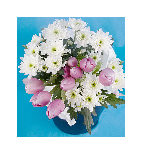
\includegraphics[width=1.8cm]{fleurs}
  \end{minipage} \\[1em]
 Combien de bouquets peut-il réaliser ? Quelle est la composition de chaque bouquet ? Donne toutes les possibilités.
\end{exercice} 

\begin{exercice}[Le pâtissier]
Un pâtissier dispose de 75 pommes, 50 oranges et 100 poires. Afin de préparer des tartes, il désire répartir ces fruits en les utilisant tous et en obtenant le maximum de tartelettes identiques. Calcule le nombre de tartelettes et indique leur composition.
\end{exercice}

\begin{exercice}[Nombres croisés]
Recopie et complète la grille à l'aide des nombres que tu trouveras grâce aux définitions.

\begin{center}
\renewcommand*\tabularxcolumn[1]{>{\centering\arraybackslash}m{#1}}
\begin{tabularx}{.6\linewidth}{|X|X|X|X|X|} 
\cline{2-5}
\multicolumn{1}{c|}{} & \cellcolor {F2} A & \cellcolor {F2} B & \cellcolor {F2} C & \cellcolor {F2} D \\\hline
\cellcolor{H1} I & \cellcolor{G3} & \cellcolor{G3} & \cellcolor{G3} & \cellcolor{Noir} \\\hline
\cellcolor{H1} II & \cellcolor{G3} & \cellcolor{G3} & \cellcolor{G3} & \cellcolor{G3} \\\hline
\cellcolor{H1} III & \cellcolor{G3} & \cellcolor{Noir} & \cellcolor{G3} & \cellcolor{G3} \\\hline
\cellcolor{H1} IV & \cellcolor{Noir} & \cellcolor{G3} & \cellcolor{Noir} & \cellcolor{G3} \\\hline
\end{tabularx}
\end{center}

\textbf{Horizontalement} :

\textcolor{H1}{\textbf{I}} : PGDC $(125 ; 250)$ ;

\textcolor{H1}{\textbf{II}} : Ce nombre est un multiple de 9 ;

\textcolor{H1}{\textbf{III}} : Le chiffre des unités d'un nombre divisible par 10 -- Ce nombre est divisible par 5 ;

\textcolor{H1}{\textbf{IV}} : Le reste de la division euclidienne de 121 par 8 -- Le quotient dans celle de 245 par 112.

\textbf{Verticalement} :

\textcolor{F2}{\textbf{A}} : Le plus petit multiple de 24 à trois chiffres ;

\textcolor{F2}{\textbf{B}} : Le quotient de la division euclidienne de 274 par 10 -- Diviseur commun à tous les entiers ;

\textcolor{F2}{\textbf{C}} : Le chiffre des centaines est 5, celui des unités 4 et c'est le PGDC $(1\,542 ; 3\,598)$ ;

\textcolor{F2}{\textbf{D}} : 3 est un diviseur de ce nombre.
\end{exercice}

%%%%%%%%%%%%%%%%%%%%%%%%Mise en page
\newpage
%%%%%%%%%%%%%%%%%%%%%%%%%%%%%%%%%%%


\begin{exercice}[Carrelage]
Dans une salle de bain, on veut recouvrir le mur se trouvant au-dessus de la baignoire avec un nombre entier de carreaux de faïence de forme carrée dont le côté est un nombre entier de centimètres, le plus grand possible. Détermine la longueur, en centimètres, du côté d'un carreau de faïence sachant que le mur mesure 210 cm de hauteur et 135 cm de largeur. Combien faudra-t-il alors de carreaux ?
\end{exercice}

\begin{exercice}[Quel est l'âge d'Aloys ?]
Aloys adore les devinettes. Lorsqu'on lui demande son âge, cette année il répond :
\begin{itemize}
 \item L'an prochain , mon âge sera divisible par 2 ;
 \item Dans deux ans , mon âge sera divisible par 3 ;
 \item Dans trois ans, mon âge sera divisible par 4 ;
 \item Dans quatre ans, mon âge sera divisible par 5 ;
 \item Et j'ai moins de 97 ans.
 \end{itemize}
Quel est l'âge d'Aloys ?
\end{exercice}


%%%%%%%%%%%%%%%%%%%%%%%%%%%%%%%%%%%%%%%%%%%%%%%%%%%%%%%%%%%%%%%%%%

\serie{Multiples communs, PPMC}

\begin{exercice}[PPMC]
Dans chaque cas, donne le PPMC :
\begin{colenumerate}{3}
 \item 2 et 6 ;
 \item 12 et 8 ;
 \item 15 et 20 ;
 \item 20 et 30 ;
 \item 18 et 24 ;
 \item 48 et 36 ;
 \item 14 et 35 ;
 \item 18 et 20 ;
 \item 36 et 60.
 \end{colenumerate}
\end{exercice}

\begin{exercice}[Jeu de cartes]
On sait d'un jeu de cartes qu’il possède un nombre de cartes qui est un multiple de 4 et de 5.
\begin{enumerate}
 \item Peut-il y avoir cinquante cartes ? vingt cartes ?
 \item Combien le paquet peut-il avoir de cartes ? Donne toutes les possibilités inférieures à 100.
 \end{enumerate}
\end{exercice}

\begin{exercice}[Quelle heure était-il ?]
A Zermatt, cinq petits bus effectuent des boucles différentes à partir de la place de la gare. Les durées des trajets sont variables suivant les bus : \\[-1em]
\begin{itemize}
 \item Ligne A : trajet de 40 minutes ;
 \item Ligne B : trajet de 20 minutes ;
 \item Ligne C : trajet de 30 minutes ;
 \item Ligne D : trajet de 10 minutes ;
 \item Ligne E : trajet de 25 minutes.
 \end{itemize}
À 16h30 , un touriste japonais reconnait les 5 bus qu'il a photographiés le matin au même endroit. \\[0.5em]
Saurais-tu dire quelle heure il était alors ?
\end{exercice}

\end{colonne*exercice}


\exercicesappr
\begin{colonne*exercice}
\begin{exercice}[Divisibilité par 4 et 100]
Un nombre est divisible par 4 si et seulement si le nombre formé par ses deux derniers chiffres est divisible par 4.\\[0.5em]
Un nombre est divisible par 100 si et seulement si ses deux derniers chiffres sont 0.\\[0.5em]
Parmi les nombres

21 ; 12 ; 2 ; 619 ; 120 ; 416 ; 296 ; 540 ; 1700,

quels sont les nombres divisibles par :
\begin{colenumerate}{2}
 \item 4 ?
 \item 100 ?
 \end{colenumerate}
\end{exercice}


\begin{exercice}[Pair]
Explique pourquoi le produit de deux entiers consécutifs est toujours pair.
\end{exercice}


\begin{exercice}[Séminaire]
Lors d'un séminaire, 324 personnes doivent se répartir dans divers ateliers. Tous les ateliers doivent avoir le même effectif, compris entre 30 et 60 personnes. Quelles sont les différentes possibilités ?
\end{exercice}


\begin{exercice}[Nombres parfaits]
\begin{enumerate}
 \item Écris la liste de tous les diviseurs de 6 ;
 \item Calcule la somme de tous ces diviseurs à l'exception de 6 ;
 \item Que remarques-tu ? On appelle nombre parfait tout entier qui a cette particularité ;
 \item Vérifie que 496 est un nombre parfait ;
 \item Trouve tous les nombres parfaits compris entre 20 et 30.
 \end{enumerate}
\end{exercice}


\begin{exercice}
Trouve les nombres entiers de trois chiffres multiples de 5 dont la somme des chiffres est 21.
\end{exercice}


\begin{exercice}[Les trois filles]
Dans une famille, il y a trois filles. La somme de leurs âges est 13 et le produit est 36.

Quel est l'âge de chaque fille ? Trouve toutes les possibilités.
\end{exercice}


\begin{exercice}[Pages]
Deux livres ont respectivement 160 et 192 pages. Chacun de ces livres est formé de fascicules ou cahiers, qui ont tous un même nombre de pages, compris entre 30 et 50.
\begin{enumerate}
 \item Quel est le nombre de pages d'un cahier ?
 \item Quel est le nombre de cahiers qui composent les deux livres ?
 \end{enumerate}
\end{exercice}


\begin{exercice}[Tempête]
Des poteaux téléphoniques étaient plantés le long d'une route, sur une ligne droite et régulièrement espacés d'un nombre entier de mètres.
Après une tempête, il n'en reste plus que trois : le premier et le dernier puis un autre situé entre les deux, à 345 m du premier et 184 m du dernier. Un technicien estime le nombre de poteaux tombés à plus de 10 mais à moins de 100 ! Combien de poteaux sont-ils tombés ?
\end{exercice}

\begin{exercice}[Arbres]
Un terrain rectangulaire mesure 168 m par 294 m. Sur ses côtés, on veut planter des arbres régulièrement espacés d'un nombre entier de mètres. Il doit y avoir un arbre à chaque coin du terrain.
Quel nombre minimum d'arbres pourra t'on planter ?
\begin{center} 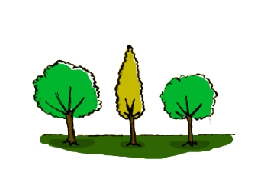
\includegraphics[width=3.3cm]{arbres} \end{center}
\end{exercice}


\begin{exercice}[Piscine]
Une piscine rectangulaire mesure 3,36 m par 7,80 m et a une profondeur de 1,44 m. On désire la carreler avec des carreaux carrés tous identiques. Le carreleur ne veut pas découper de carreaux mais préfère les grands carreaux, plus faciles à poser. Son fournisseur a toutes les tailles de carreaux en nombre entier de centimètres.
\begin{enumerate}
 \item Quelle taille de carreaux doit-il commander ? Prendre la plus grande mesure possible.
 \item Son fournisseur vend les carreaux par lot de 100. Combien de lots doit-il commander ?
 \end{enumerate}
\end{exercice}


\begin{exercice}[Sacrée collection !]

\vspace{1em}

\begin{minipage}[c]{0.65\linewidth}
Abdel dit à Doris : « J'ai plus de 400 DVD mais moins de 450 !

En les groupant par 2 ou par 3 ou par 4 ou par 5, c'est toujours la même chose, il m'en reste un tout seul ! ».
 \end{minipage} \hfill%
 \begin{minipage}[c]{0.32\linewidth}
  \begin{center} 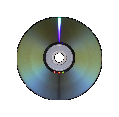
\includegraphics[width=1.4cm]{CD} \end{center}
  \end{minipage} \\
Combien Abdel a-t-il de DVD ?
\end{exercice}



%%%%%%%%%%%%%%%%%%%%%%%%%%%%%%%%Mise en page
\newpage
%%%%%%%%%%%%%%%%%%%%%%%%%%%%%%%%%%%%%%%%%%%%




\begin{exercice}[Escalier]
Le nombre de marches d’un escalier est compris entre 40 et 80 :
\begin{itemize}
 \item Si on compte ces marches deux par deux, il en reste une ;
 \item Si on les compte trois par trois, il en reste deux ;
 \item Si on les compte cinq par cinq, il en reste quatre.
 \end{itemize}
Quel est le nombre de marches de cet escalier ?
\end{exercice}


\begin{exercice}[La numération moderne]
$3 \cdot 10^3 + 2 \cdot 10^2 + 8 \cdot 10^1 + 4 \cdot 10^0$ est la décomposition en base « dix » de 3\,284. Décompose les nombres 5\,348 et 4\,367 \,214 en base « dix ».
\end{exercice}


\begin{exercice}[Les limites de la calculatrice]
\begin{enumerate}
 \item Avec la calculatrice, donne un ordre de grandeur du produit de 987\,654 par 876\,534 ;
 \item Calcule le résultat exact de ce produit.
 \end{enumerate}
\end{exercice}


\begin{exercice}[L'unité d'enregistrement informatique]
En informatique, on utilise une unité d'enregistrement appelée « octet ».
\begin{enumerate}
 \item Calcule avec ta calculatrice la valeur des expressions suivantes :
 \begin{itemize}
  \item $A = 2^{10}$ octets ;
  \item $B = 2^{20}$ octets ;
  \item $C = 2^{30}$ octets.
  \end{itemize}
 \item Explique pourquoi l'expression $A$ est généralement appelée « 1 kilooctet ». On note $A \approx 1$ ko ($10^3$ octets). Par approximation, on écrit $A = 1$ ko.
 \item De même $B$ est appelé « 1 Mégaoctet » (1 Mo) et $C$ « 1 Gigaoctet » (1 Go). Indique par quelles puissances de 10, se traduisent les préfixes « méga » et « giga ». 
 \end{enumerate}
\end{exercice}


\begin{exercice}[Multiple et diviseur]
\begin{enumerate}
 \item À l'aide de la calculatrice retrouve les nombres entiers positifs non nuls $n$, $m$ et $p$ tels que :
 
 \begin{center} $349\,272 = 2^n \cdot 3^m \cdot 7^p \cdot 11$ \end{center}

 \item À l'aide de la calculatrice retrouve les nombres entiers positifs non nuls $r$, $s$ et $t$ tels que :
 
 \begin{center} $36\,288 = 2^r \cdot 3^s \cdot 7^t$ \end{center}
 
 \item On considère : $N = 2^3 \cdot 3^3 \cdot 7$.
 
Sans calculer la valeur de $N$, montre que $N$ est un diviseur commun à 349\,272 et à 36\,288.

 \item On considère : $M = 2^6 \cdot 3^4 \cdot 7^2 \cdot 11$.
 
Sans calculer la valeur de $M$, montre que $M$ est un multiple commun à 349\,272 et à 36\,288.
 \end{enumerate}
\end{exercice}


\begin{exercice}[Chemin de diviseurs\ldots]
\begin{center} 
\begin{tikzpicture}[scale=1,every node/.style={scale=1}]

\tikzset{noeud/.style={minimum width=1cm,minimum height=1cm,rounded corners=4pt,draw,rectangle,color=G1,fill=G1!10,text=black,scale=1}}

\foreach \x / \y / \val in {0/0/10,3/0.3/13,1/0.8/31,2/1/41,4.5/0.8/47,5.7/1.4/44,0/2/6,0.8/2.2/7,2.5/2.2/23,5.2/2.1/32,1.3/3/43,2.6/3.2/11,0/3.5/39,1.9/3.9/64,4/3/3,6.3/3.4/19,1/4.5/130,3/4.8/121,4/4.2/17,4.9/4.5/53,5.7/4.1/28,0.2/5.4/16,4.4/5.6/35,5.5/5.7/110,6.5/5.4/17,1.2/6.2/9,2.8/6.4/49,6.5/6.5/4}
{\node at(\x,\y) {\val};
\node[below=3pt] at(\x,\y) {$\bullet$};}


%Les 2 noeuds de départ et d'arrivée :
\node[noeud] at(6.5,0) {15};
\node[below=3pt] at(6.5,0) {$\bullet$};

\node[noeud] at(0,6.5) {14};
\node[below=3pt] at(0,6.5) {$\bullet$};

\end{tikzpicture}

\end{center}

Sur la figure ci-dessus, trouver un chemin qui mène de 14 à 15 en alternant multiples et diviseurs. Pour vous aider, continuer le raisonnement suivant : \\[1em]
Je relie 14 à 28 car 28 est un multiple de 14 ;

Je relie 28 à \ldots \ldots car \ldots \ldots est un diviseur de 28 ;

Je relie \ldots à \ldots \ldots car \ldots \ldots est un multiple de \ldots \ldots ;

Je relie \ldots à \ldots \ldots car \ldots \ldots est un diviseur de \ldots \ldots ;

Je relie \ldots à \ldots \ldots car \ldots \ldots est un multiple de \ldots \ldots ;

Je relie \ldots à \ldots \ldots car \ldots \ldots est un diviseur de \ldots \ldots ;

Je relie \ldots à \ldots \ldots car \ldots \ldots est un multiple de \ldots \ldots ;

Je relie \ldots à \ldots \ldots car \ldots \ldots est un diviseur de \ldots \ldots ;

Je relie \ldots à \ldots \ldots car \ldots \ldots est un multiple de \ldots \ldots ;

Je relie \ldots à \ldots \ldots car \ldots \ldots est un diviseur de \ldots \ldots ;

Je relie \ldots à 15 car \ldots \ldots est un multiple de 15.

Tous les nombres du tableau ne sont pas utilisés.

\end{exercice}



%%%%%%%%%%%%%%%%%%%%%%%%%%%%%%%%Mise en page
\newpage
%%%%%%%%%%%%%%%%%%%%%%%%%%%%%%%%%%%%%%%%%%%%





\begin{exercice}[Chemin premier\ldots]
Trouver le chemin qui mène de la case $X$ à la case $Y$ en passant par 13 cases (sans compter les cases $X$ et $Y$) contiguës différentes contenant chacune un nombre premier.

\begin{center} 
\begin{tikzpicture}[scale=0.7]%Attention : si on change le scale, il faut aussi le changer dans le \tikset
\tikzset{noeud/.style={minimum width=1cm,minimum height=1cm,draw,rectangle,color=G1,rounded corners=4pt,fill=G1!10,text=black,scale=0.7}}

\foreach \a/\n in {0/97,1/89,2/83,4/71,5/83,6/97}{\node[noeud] at (0.5+\a*1.5,0.5){\n};}

\foreach \a/\n in {0/61,1/43,2/21,3/31,4/41,5/59,6/73}{\node[noeud] at (0.5+\a*1.5,2){\n};}

\foreach \a/\n in {0/13,1/93,2/47,3/89,4/27,5/53,6/67}{\node[noeud] () at (0.5+\a*1.5,3.5){\n};}

\foreach \a/\n in {0/19,1/59,2/81,3/79,4/41,5/89,6/91}{\node[noeud] () at (0.5+\a*1.5,5){\n};}

\foreach \a/\n in {0/29,1/57,2/61,3/47,4/63,5/13,6/23}{\node[noeud] at (0.5+\a*1.5,6.5){\n};}

\foreach \a/\n in {0/43,1/67,2/49,3/17,4/51,5/17,6/11}{\node[noeud] at (0.5+\a*1.5,8){\n};}

\foreach \a/\n in {0/37,1/23,2/11,4/79,5/31,6/19}{\node[noeud] at (0.5+\a*1.5,9.5){\n};}

%%%% Les traits entre cases :
\foreach \a in {0,1.5,...,7.5} {\foreach \b in {0,1.5,...,9}{\draw [blue] (\a+1,\b+0.5)--(\a+1.5,\b+0.5);}}
\foreach \a in {0,1.5,...,9} {\foreach \b in {0,1.5,...,7.5}{\draw [blue](\a+0.5,\b+1)--(\a+0.5,\b+1.5);}}

%%% Les deux cases de départ et d'arrivée

\node[minimum width=1cm,minimum height=1cm,draw,rectangle,color=F1,rounded corners=4pt,fill=F1!10,text=F1,scale=0.7] at (5,0.5){Y};
\node[minimum width=1cm,minimum height=1cm,draw,rectangle,color=F1,rounded corners=4pt,fill=F1!10,text=F1,scale=0.7] at (5,9.5){X};
\end{tikzpicture}
\end{center}

\begin{center} 
\textbf{Liste des nombres premiers inférieurs à 1000 :}
\vspace{1em}

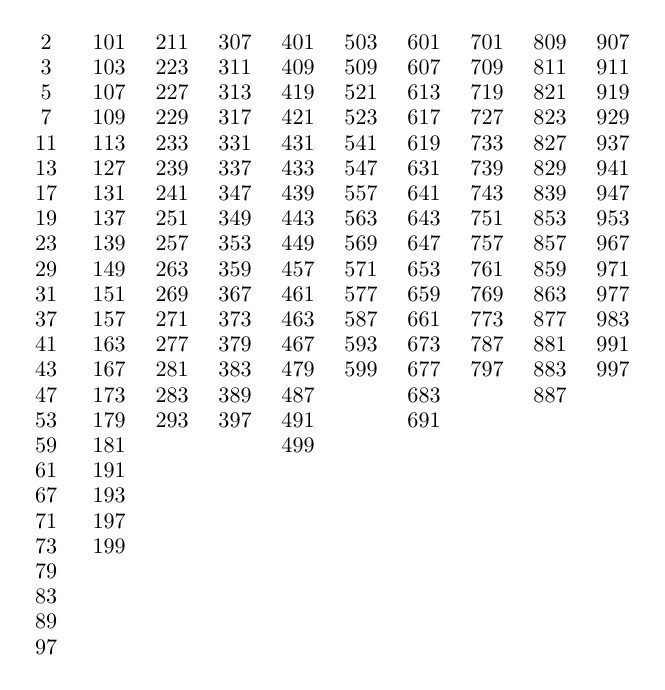
\begin{tikzpicture}[scale=0.8,every node/.style={scale=.8}]
\foreach \a/\b in {0/2,1/3,2/5,3/7,4/11,5/13,6/17,7/19,8/23,9/29,10/31,11/37,12/41,13/43,14/47,15/53,16/59,17/61,18/67,19/71,20/73,21/79,22/83,23/89,24/97}{ \node () at (0.5,-0.4*\a){\b};}

\foreach \a/\b in {0/101,1/103,2/107,3/109,4/113,5/127,6/131,7/137,8/139,9/149,10/151,11/157,12/163,13/167,14/173,15/179,16/181,17/191,18/193,19/197,20/199}{ \node () at (1.5,-0.4*\a){\b};}

\foreach \a/\b in {0/211,1/223,2/227,3/229,4/233,5/239,6/241,7/251,8/257,9/263,10/269,11/271,12/277,13/281,14/283,15/293}{ \node () at (2.5,-0.4*\a){\b};}

\foreach \a/\b in {0/307,1/311,2/313,3/317,4/331,5/337,6/347,7/349,8/353,9/359,10/367,11/373,12/379,13/383,14/389,15/397}{ \node () at (3.5,-0.4*\a){\b};}

\foreach \a/\b in {0/401,1/409,2/419,3/421,4/431,5/433,6/439,7/443,8/449,9/457,10/461,11/463,12/467,13/479,14/487,15/491,16/499}{ \node () at (4.5,-0.4*\a){\b};}

\foreach \a/\b in {0/503,1/509,2/521,3/523,4/541,5/547,6/557,7/563,8/569,9/571,10/577,11/587,12/593,13/599}{ \node () at (5.5,-0.4*\a){\b};}

\foreach \a/\b in {0/601,1/607,2/613,3/617,4/619,5/631,6/641,7/643,8/647,9/653,10/659,11/661,12/673,13/677,14/683,15/691}{ \node () at (6.5,-0.4*\a){\b};}

\foreach \a/\b in {0/701,1/709,2/719,3/727,4/733,5/739,6/743,7/751,8/757,9/761,10/769,11/773,12/787,13/797}{ \node () at (7.5,-0.4*\a){\b};}

\foreach \a/\b in {0/809,1/811,2/821,3/823,4/827,5/829,6/839,7/853,8/857,9/859,10/863,11/877,12/881,13/883,14/887}{ \node () at (8.5,-0.4*\a){\b};}

\foreach \a/\b in {0/907,1/911,2/919,3/929,4/937,5/941,6/947,7/953,8/967,9/971,10/977,11/983,12/991,13/997}{ \node () at (9.5,-0.4*\a){\b};}

\end{tikzpicture}
\end{center}
\end{exercice}

\prof{pour les très bons élèves; exercice de renforcement}
\begin{exercice}[La division euclidienne]
Euclide est un mathématicien de la Grèce antique. De son nom est tiré la division euclidienne, la géométrie euclidienne et l'algotithme d'Euclide. Ce dernier peut également servir au calcul du PGDC.\\
Prenons l'exemple du PGDC de 315 et 600.\\
On pose $600\div315=1$ reste 285.\\
On poursuit ainsi $315\div285=1$ reste 30.\\
$285\div30=9$ reste \textcolor{red}{15}.\\
$30\div15=2$ reste 0. On s'arrête car le reste est nul.\\
Le PGDC(315;600)=\textcolor{red}{15}
\\
\\
En utilisant l'algorithme d'Euclide, calcule le PGDC des nombres suivants:

\begin{colenumerate}{2}
 \item 78 et 182
 \item 135 et 210
 \item 375 et 675
 \item 352 et 682
\end{colenumerate}
\end{exercice}

\end{colonne*exercice}

\connaissances

\QCMautoevaluation{Pour chaque question, plusieurs réponses sont
  proposées.  Déterminer celles qui sont correctes.}

\begin{QCM}
  \begin{GroupeQCM} 
    \begin{exercice}
      84 est divisible par \ldots
      \begin{ChoixQCM}{4}
      \item 5
      \item 9
      \item 2
      \item3
      \end{ChoixQCM}
\begin{corrige}
     \reponseQCM{cd} 
   \end{corrige}
    \end{exercice}

    \begin{exercice}
      150 est divisible par \ldots
      \begin{ChoixQCM}{4}
      \item 3
      \item 2
      \item 5
      \item 10
      \end{ChoixQCM}
\begin{corrige}
     \reponseQCM{abcd}
   \end{corrige}
    \end{exercice}
    
    \begin{exercice}
      435 est \ldots
      \begin{ChoixQCM}{4}
      \item Un multiple de 5
      \item Un diviseur de 5
      \item Divisible par 5
      \item Un multiple de 3
      \end{ChoixQCM}
\begin{corrige}
     \reponseQCM{acd}
   \end{corrige}
    \end{exercice}

    \begin{exercice}
      17 est \ldots
      \begin{ChoixQCM}{4}
      \item Un diviseur de 3\,672
      \item Un multiple de 17
      \item Le seul diviseur de 17
      \item Un multiple de 8,5
      \end{ChoixQCM}
\begin{corrige}
     \reponseQCM{abd}
   \end{corrige}
    \end{exercice}

    \begin{exercice}
      Retrouve la (ou les) affirmation(s) vraie(s) :
      \begin{ChoixQCM}{4}
      \item Tout nombre entier est un multiple de 0
      \item Il existe toujours au moins un diviseur commun à deux entiers
      \item La liste des diviseurs d'un entier est infinie
      \item Un nombre entier est toujours divisible par lui‑même
      \end{ChoixQCM}
\begin{corrige}
     \reponseQCM{bd}
   \end{corrige}
    \end{exercice}
    
    \begin{exercice}
      15 est \ldots
      \begin{ChoixQCM}{4}
      \item Un diviseur commun à 30 et 45
      \item Le PGDC de 30 et 45
      \item Le plus grand multiple commun à 3 et 5
      \item Le plus grand des diviseurs communs à 60 et 135
      \end{ChoixQCM}
\begin{corrige}
     \reponseQCM{abd}
   \end{corrige}
    \end{exercice}
    
    \begin{exercice}
      Le PGCD de 12 et 18 est \ldots
      \begin{ChoixQCM}{4}
      \item 1
      \item 6
      \item 2
      \item 0
      \end{ChoixQCM}
\begin{corrige}
     \reponseQCM{b}
   \end{corrige}
    \end{exercice}

    \begin{exercice}
      24 est \ldots
      \begin{ChoixQCM}{4}
      \item Le PPMC de 6 et 4
      \item Un multiple commun à 8 et 6 
      \item Le PPMC de 8 et 6
      \item Un multiple de 48
      \end{ChoixQCM}
\begin{corrige}
     \reponseQCM{bc}
   \end{corrige}
    \end{exercice}
   
\end{GroupeQCM}
\end{QCM}

     



\begin{QCM}
  \begin{GroupeQCM} 

    \begin{exercice}
      $5^3 =$ \ldots
      \begin{ChoixQCM}{4}
      \item 15
      \item 8
      \item 125
      \item $03:05:00$
      \end{ChoixQCM}
\begin{corrige}
     \reponseQCM{c}
   \end{corrige}
    \end{exercice}
    
    \begin{exercice}
      51 est \ldots
      \begin{ChoixQCM}{4}
      \item Un nombre premier
      \item Un multiple de 7
      \item Divisible par 17
      \item Un diviseur de 102
      \end{ChoixQCM}
\begin{corrige}
     \reponseQCM{cd}
   \end{corrige}
    \end{exercice}
    
    \begin{exercice}
      Dans $4^3$, 3 est \ldots
      \begin{ChoixQCM}{4}
      \item La base
      \item L'exposant
      \item La puissance
      \item Le facteur
      \end{ChoixQCM}
\begin{corrige}
     \reponseQCM{bc}
   \end{corrige}
    \end{exercice}
    
    \begin{exercice}
      La décomposition en produits de facteurs premiers de 84 possède \ldots
      \begin{ChoixQCM}{4}
      \item 3 facteurs distincts
      \item Le facteur $2^3$
      \item 4 facteurs
      \item Deux facteurs premiers
      \end{ChoixQCM}
\begin{corrige}
     \reponseQCM{ac}
   \end{corrige}
    \end{exercice}
    
\end{GroupeQCM}
\end{QCM}

  


\TravauxPratiques % pour nous "travailler en groupe"

\begin{TP}[Méthode géométrique de calcul du PGDC]

\partie{Découverte de la méthode}
Dans cette partie, nous allons illustrer le calcul du PGDC de 18 et 22 par une figure géométrique.\\[0.5em]
On commence par construire un rectangle $ABCD$ tel que $AB = 18$ et $BC = 22$. On construit ensuite le carré $ABEF$. Dans la surface restante représentée par le rectangle $ECDF$, on peut placer quatre carrés de côté $EC$. On construit ensuite le carré $JLMF$ et on constate que la surface restante est l'intérieur d'un carré : \textcolor{C2}{$LKDM$}.
\begin{center} 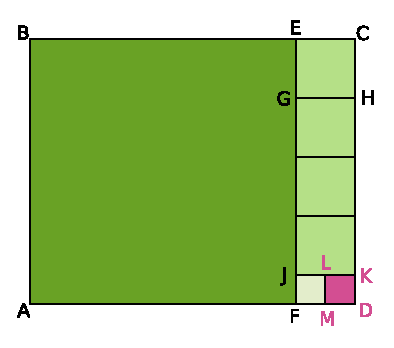
\includegraphics[width=5.7cm]{methode_geometrique} \end{center}

\begin{enumerate}
 \item Chaque membre du groupe reproduit cette figure en choisissant un carreau ou 1 cm comme unité ;
 \item Chaque membre calcule le PGDC de 18 et 22 ;
 \item À quelle longueur correspond le PGDC de 18 et 22 ?
 \end{enumerate}
 
\partie{Quelques autres exemples}

\begin{enumerate}
 \item Chaque membre détermine le PGDC de 12 et 45 par la méthode géométrique (sur une feuille à petits carreaux) ;
 \item Chaque membre vérifie son résultat en calculant le PGDC de 12 et 45 par la méthode des soustractions successives ;
 \item Chaque membre choisit un nombre entre 10 et 20 et un autre nombre entre 40 et 50. Il donne ses deux nombres à son voisin de droite qui doit déterminer leur PGDC par la méthode géométrique (sur une feuille à carreaux).
 \end{enumerate}
 
\end{TP}

%%%%%%%%%%%%%%%%%%%%%%%%%%%%%%%%%%%%%%%%%%%%%%%%%%%%%%%%%%%%%%%%%%%

\begin{TP}[Dans le coeur des micros]

\partie{Parlons chiffre}

En informatique, on utilise seulement des 0 et des 1 pour coder les nombres. On travaille avec un système de numération binaire.

\begin{center}
\begin{tabularx}{0.7\linewidth}{|X|X|c|}
\hline
Écriture binaire & Écriture décimale & Lien entre les deux écritures \\ \hline
1 & 1 & $1\cdot 2^0$ \\ \hline
10 & 2 & $1\cdot2^1+0\cdot 2^0$ \\ \hline
11 & 3 & $1\cdot2^1+1\cdot 2^0$ \\ \hline
100 & 2 & $1\cdot2^2+0\cdot 2^1+0\cdot 2^0$ \\ \hline
\end{tabularx} \\
\end{center}

\begin{enumerate}
 \item Observez bien la table de correspondance précédente puis déterminez l'écriture en binaire des entiers inférieurs à 10 ; \label{NbsEntMultDivis_engroupe}
 \item Reproduisez la feuille de calcul suivante sur un tableur : \\[1em]
 \begin{center}
 \begin{tabularx}{0.7\linewidth}{|X|X|X|X|X|X|X|X|X|}
 \hline
 \rowcolor{Gris2} & A & B & C & D & E & F & G & H \\ \hline
 \cellcolor{Gris2} 1 & \multicolumn{5}{l|}{Nombre en binaire}  & & & \\ \hline 
 \cellcolor{Gris2} 2 & 0 & 1 & 1 & 1 & 1 & 1 & 0 & 1 \\ \hline
 \cellcolor{Gris2} 3 & \multicolumn{7}{l|}{Nombre en écriture décimale} & \ldots  \\ \hline 
 \end{tabularx} \\
 \end{center}
 
 \vspace{1em}
 
 Programmez en H$3$ le calcul nécessaire pour obtenir l'écriture décimale d'un nombre en binaire.
  \end{enumerate}
  
  
 \partie{La table ASCII}
 L'unité d'enregistrement en informatique est le \textbf{bit}, symbolisé par un 0 ou un 1. Un \textbf{octet} correspond à une suite de huit bits, par exemple 0100 1101.
 
 \begin{enumerate}
 \item Combien de nombres peut-on écrire avec un octet ? \\[0.75em]
Pour coder la centaine de caractères présents sur un clavier, on les numérote de 0 à 255 et on les code à l'aide d'un octet. La table qui permet de mettre en correspondance un caractère et le nombre entre 0 et 255 s'appelle la \textbf{table ASCII}. Récupérez-la sur Wikipedia.
 
 \item Retrouvez l'écriture décimale du nombre 0100 0001. À quelle lettre correspond-il ?
 \item À l'aide de la question \textbf{\ref{NbsEntMultDivis_engroupe}}, retrouvez l'écriture en binaire des codes des autres lettres de l'alphabet.\\[0.75em]
Choisissez alors quatre mots de moins de dix lettres, codez-les en binaire puis demandez aux autres groupes de les retrouver. Faites de même avec les mots qui vous auront été donnés.
 \end{enumerate}
\end{TP}

%%%%%%%%%%%%%%%%%%%%%%%%%%Mise en page

\vspace*{3cm}

\phantom{Pour sauter une ligne}

%%%%%%%%%%%%%%%%%%%%%%%%%%%%%%%%%%%%%%




\pagebreak

\recreation
\begin{enigme}[Nombres triangulaires]

Ci-dessous, les cinq premiers nombres « triangulaires » :

\begin{center} 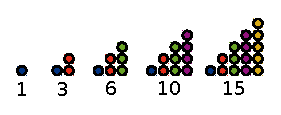
\includegraphics[width=5cm]{billes} \end{center} 

\begin{enumerate}
 \item Quel est le millième ?
 \item Que remarques-tu lorsque tu additionnes deux nombres triangulaires consécutifs ? 
 \end{enumerate}
 
 \end{enigme}
 
 \vspace*{2em}

\begin{enigme}[Geôle]
Dans un donjon, vingt cellules numérotées de 1 à 20 sont fermées à clé. Ces cellules s'ouvrent et se ferment en un tour de clé.

Alors que les prisonniers dorment à poings fermés, un premier gardien, les pensant ouvertes, met un tour de clé à toutes les cellules.

Peu après, un deuxième gardien met un tour de clé à toutes les cellules dont le numéro est multiple de 2.

Arrive ensuite un troisième gardien qui met un tour de clef à toutes les cellules dont le numéro est un multiple de 3 !

Et ainsi de suite...

Au final, vingt gardiens se sont succédés !

\begin{enumerate}
 \item Quels sont les numéros des cellules dont les prisonniers vont facilement pouvoir s'évader ?
 \end{enumerate}
 
\emph{Reprends le même problème avec 500 cellules et 500 passages de gardiens !! Justifie ta réponse.}
\end{enigme} 



